\documentclass{beamer}

\usepackage[utf8]{inputenc}
\usepackage[T1]{fontenc}
\usepackage{microtype}
\usepackage[german]{babel}
\usepackage{hyperref}
\usepackage{lmodern}
\usepackage{wasysym}
\usepackage{textpos}
\usepackage{epstopdf}
\usepackage[pageofpages=von,
            titlepagelogo=resource/logo]{beamerthemeUhh}
\usepackage{beamercolorthemeuhh}

\usepackage{tikz}
\usepackage{setspace}

\newenvironment{changemargin}[2]{%
\begin{list}{}{%
\setlength{\topsep}{0pt}%
\setlength{\leftmargin}{#1}%
\setlength{\rightmargin}{#2}%
\setlength{\listparindent}{\parindent}%
\setlength{\itemindent}{\parindent}%
\setlength{\parsep}{\parskip}%
}%
\item[]}{\end{list}}

\logo{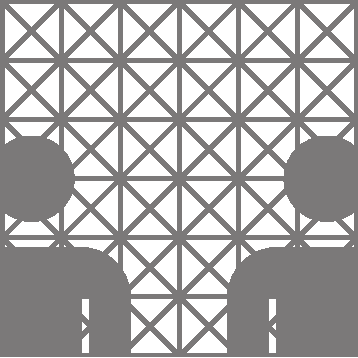
\includegraphics[height=0.125\paperheight]{resource/logo-fbi}}

\setbeamertemplate{frametitle continuation}[from second][]
\usefonttheme{professionalfonts}	

%%%%%
\newcommand{\myName}{Felix Favre}
\newcommand{\myEmail}{1favre@informatik.uni-hamburg.de}
\newcommand{\myTitle}{Validierung von dynamisch geladenem Javascript Codes in Webapplikationen}
\newcommand{\myKeywords}{}
\institute{Universität Hamburg -- Fachbereich Informatik -- Abschlussarbeiten Seminar}
\date[15.04.2015]{22. April 2015}


\title{\myTitle}
\author{\myName}
\keywords{\myKeywords}
\subject{}

\definecolor{uhh}{RGB}{226,0,26}

\hypersetup{ 
	pdftitle={\myTitle},
	pdfauthor={\myName},
	pdfkeywords={\myKeywords}, 
	bookmarksnumbered=true,
	bookmarksopen=true,
	bookmarksopenlevel=1,
	colorlinks=true,
	linkbordercolor={1 1 1},
	urlcolor=uhh,
	anchorcolor=black,
	linkcolor=black,
	citecolor=black,
	filecolor=black,
	menucolor=black
}

\pdfcompresslevel=9
\pdfimageresolution=72
\pdfpkresolution=72

\newcommand{\maxFrameImage}[1]{
\begingroup
\setbeamercolor{background canvas}{bg=black}
\begin{frame}[plain]
\begin{changemargin}{-1cm}{-1cm}
\begin{center}
\includegraphics[width=\paperwidth,height=\paperheight,keepaspectratio]
{#1}
\end{center}
\end{changemargin}
\end{frame}
\endgroup
}

\begin{document}

\pdfbookmark[2]{Titelseite}{title}
{
    \usebackgroundtemplate{
\includegraphics[width=\paperwidth]{resource/uhh-bg.png}}
    \frame{  
        \titlepage
    }
}

\begin{frame}{Über mich}
  \begin{itemize}
    \item Felix Favre
    \item 8. Semester Bsc. Informatik
    \item Aktueller Fokus: Webentwicklung und Security
    \pause
    \item Studiere Teilzeit -> Bachelorarbeit noch nicht in Sicht
    \item Hypothetisches Expose für dieses Seminar
  \end{itemize}
\end{frame}

\begin{frame}{Status}
  \begin{itemize}
    \item Themengebiet aus aktuellem Fokus abgeleitet
    \item Meiner Meinung nach ein akutes Problem
    \item Aktuellen technischen Status recherchiert
    \item Gedanken über Lösungsansätze gemacht
  \end{itemize}
\end{frame}

\begin{frame}{The End}
  \begin{itemize}
    \item Danke an Tim für das Theme!
    \item Fragen?
    \item Anmerkungen?
  \end{itemize}
\end{frame}

\end{document}

